\section{实现与信息访问}\label{app:implementation}

\paragraph{物理模型。}
状态向量为 $(h_1,h_2,h_3,T_{m1},T_{m2},T_{m3},r_b,m_{\ell1},m_{\ell2},d_{sw1},d_{sw2})$。
温度—焓关系使用表格化 IAPWS 物性网格。观测映射读取物理状态和给定边界，没有独立的神经均值温度头。
稳态锚点由物理观测反演得到，融合模型只修正金属温度和燃料滞后；三个蒸汽焓、两个液体存量、两个喷水输运状态保留锚定初值。
均值修正幅度受固定状态尺度的 0.1 倍限制；观察器输出头零初始化时严格回到锚点。
每个 10 秒采样步由五个 2 秒子步组成。每个子步都用当前状态重新计算闭合项，式~\ref{eq:trans}省略了该内部组合。

\paragraph{闭合项的限制。}
两隐层 tanh MLP 输出三个分段有界功率修正。保守注入在蒸汽/金属两侧以正负配对形式加入。
输入是归一化物理状态和六个允许的基础边界，排除实测喷水总量。本轮没有额外潜变量或随机闭合项输入。
输入排除只是一项直接接口约束：状态本身已经受较早动作影响。令动作扰动下的状态灵敏度为 $S_k=\partial x_k/\partial\epsilon$，局部链式法则包含
\[
S_{k+1}=(\Phi_x+\Phi_r r_x)S_k+\Phi_u\,
\frac{\partial u_{k+1}}{\partial\epsilon},\qquad S_t=0.
\]
学习闭合项仍能通过状态修改灵敏度。正负功率注入限制残差作用位置，但不证明参数可辨识、所有工况下稳定或真实增益恢复。

\paragraph{观察器候选。}
两种观察器隐藏宽度均为 128。候选对 23 个历史变量分别以长度 16、步长 8 分块，每变量 11 块，共 253 个 token。
线性分块嵌入加变量和位置嵌入，经过一层四头 Transformer 编码器；11 个学习状态查询再交叉注意到其输出。
逐状态修正头同时读取查询特征与压力特征。GRU 和候选共享修正上界、状态掩码、物理转移、闭合项、历史扩展和种子对应的训练抽样。
token 不读取未来历史；它替换的是观察器，而不是以注意力端到端替换物理动力学。

\paragraph{黑箱。}
黑箱借鉴变量 token 预测~\cite{liu2024itransformer}：用 96 到 64 的线性映射嵌入每个历史变量，用独立的 18 到 64 映射嵌入每个未来通道（2 阀位、7 边界）。
32 个 token 经过两层四头 Transformer，再由展平线性头预测相对历史主汽温均值的 18 步偏差。dropout 为 0.1，前馈宽度 128。
这是本地适配基线，不是原始 benchmark 架构或物理引导主汽温模型~\cite{zhang2026sst}的原样复现。

\begin{table}[!ht]
\centering\small
\begin{tabular}{lrrrr}
\toprule
项目 & 黑箱 & 灰箱 & GRU 融合 & Token 融合\\
\midrule
消费历史扩展数 & 9 & 0 & 9 & 9\\
学习观察器 & --- & --- & GRU & 分块/查询\\
神经功率闭合项 & --- & 无 & 保守注入 & 保守注入\\
再润湿 & --- & 启用 & 消融 & 消融\\
接收梯度的参数数 & 111,250 & 99 & 65,808 & 278,248\\
更新上限 & 3,000 & 24,000 & 24,000 & 24,000\\
Batch size & 128 & 32 & 32 & 32\\
验证间隔（更新数） & 500 & 200 & 200 & 200\\
Patience（验证次数） & 3 & 20 & 20 & 20\\
\bottomrule
\end{tabular}
\caption{实际执行配置，而非容量/算力匹配 benchmark。活跃参数数排除已实例化但被旁路的网络；结构模型的观测不确定性参数可经 NLL 接收梯度。}
\end{table}

\section{数据合同、估计量和溯源}\label{app:stats}

7 个基础通道为蒸汽流量、给煤指令、分离器压力、分离器温度、给水温度、出口压力、喷水总量。
9 个扩展为修正燃料、投运磨煤机数、加权磨煤机气温、烟气氧量、总二次风、再热器 A/B 侧入口烟温、水煤比、机组负荷。
扩展只参与历史，不向任何模型提供未来扩展。水煤比在此是协变量，不是额外的物理功率修正；没有特征消融，不能分离其独立收益。

物理模型对基础通道使用固定工程尺度；扩展使用共同的训练行均值和标准差。黑箱所有历史通道使用训练统计量，输出以历史目标均值为偏置；给定未来基础协变量不经过该历史归一化。
未来喷水总量对黑箱可见，对动作驱动物理模型被忽略。阀位变化时保持这一通道不变，是诊断输入定义，不代表自洽的现场反事实。因此应按完整方法比较理解结果。

训练从固定的、带放回抽取的 20,000 窗口库中抽样。训练库、验证、响应 manifest 随机种子分别为 15,000、30,000、60,000。
训练种子控制初始化和后续 minibatch。所有模型的验证目标、时间标记和起点完全一致；所有探针共享起点、阀位剂量和支持域掩码。
256 个预测窗口、64 个响应历史均覆盖 13 个 UTC 日。窗口可以重叠，不将窗口视为独立实验单元。

每个种子的配对 H18 误差差值先在 UTC 日内平均，再对 13 个日均值带放回抽样 1,000 次，RNG 种子为 11,000，取 2.5/97.5 百分位区间。
响应曲线逐点采用相同流程。这些区间描述选定检查点条件下的日间变化，没有校正检查点选择、此前验证复用、多重比较或跨日序列依赖。
三个种子不是三台独立电厂；图中阴影则是三个种子的日均值最小—最大范围。

\begin{table}[!ht]
\centering\small
\begin{tabular}{lccc}
\toprule
H18 候选减参考（\degc{}） & 种子 0 & 种子 1 & 种子 2\\
\midrule
GRU $-$ 黑箱 & $0.068$ & $0.046$ & $0.104$\\
95\% 日块区间 & $[0.027,0.108]$ & $[-0.002,0.093]$ & $[0.067,0.137]$\\
GRU $-$ 灰箱 & $-0.537$ & $-0.541$ & $-0.500$\\
95\% 日块区间 & $[-0.784,-0.318]$ & $[-0.756,-0.341]$ & $[-0.725,-0.299]$\\
Token $-$ GRU & $0.267$ & $0.212$ & $0.154$\\
95\% 日块区间 & $[0.210,0.329]$ & $[0.155,0.269]$ & $[0.119,0.193]$\\
\bottomrule
\end{tabular}
\caption{从保存数组独立复算的配对描述性区间，不作经选择校正或确认性显著性声明。}
\end{table}

注册支持检查将每个阀位历史边际最小/最大值向外扩 0.05，并检查基线与干预序列。本轮两个阀门的 64 个历史全部通过，没有丢弃历史。
这个宽松的轴对齐检查不检验联合状态—动作支持、条件激励或保持边界不变的现实合理性；因此 supported-only 曲线与主曲线完全相同，不另画重复附图。

\paragraph{产物审计。}
回传包含 12 个检查点、训练 ledger 和 24 个预测/响应原始数组。本地只读审计验证产物哈希、检查点与输入身份绑定、共同索引配对。
独立数组归约检查代码指纹，重算每条预测曲线、响应曲线及配对区间，恢复相同融合模型选择。输入、映射、物性网格指纹保存在内部审计记录。
执行侧回传记录声称完成 24 组推理数组重放；本次写稿没有从原始现场记录独立再做推理重放。没有为初稿训练或访问 test。
审计确认回传证据的一致性，不确认未测量的现场干预响应真值。

\section{观察器选择与逐种子诊断}\label{app:ablation}

\begin{figure}[!ht]
\centering
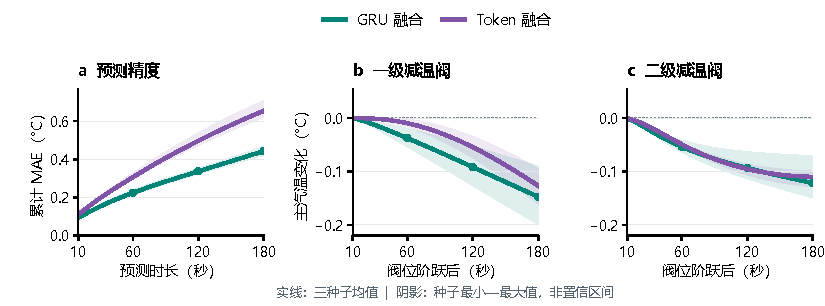
\includegraphics[width=\linewidth]{figures/figS1_observer_ablation_zh.pdf}
\caption{\textbf{Token 观察器不晋级。}物理配置、历史合同和评估 manifest 相同，仅观察器架构变化。三个种子的 token H18 预测误差均高于 GRU，两者均有负向平均末端响应；响应不参与选模。实线和阴影定义与图~\ref{fig:evidence}相同。}
\end{figure}

\begin{table}[!ht]
\centering\small
\begin{tabular}{lrrrr}
\toprule
方法 / 种子 & H18 MAE & 阀 1 H18 & 阀 2 H18 & 最佳更新\\
\midrule
纯黑箱 / 0 & 0.3735 & $+0.000013$ & $+0.001335$ & 3,000 \\
纯黑箱 / 1 & 0.3756 & $-0.000025$ & $+0.000678$ & 2,500 \\
纯黑箱 / 2 & 0.3628 & $+0.000305$ & $+0.000183$ & 3,000 \\
纯灰箱 / 0 & 0.9787 & $+0.004601$ & $+0.032581$ & 23,800 \\
纯灰箱 / 1 & 0.9623 & $+0.004401$ & $+0.033384$ & 24,000 \\
纯灰箱 / 2 & 0.9668 & $+0.004435$ & $+0.033175$ & 24,000 \\
GRU 融合 / 0 & 0.4414 & $-0.198801$ & $-0.145255$ & 21,000 \\
GRU 融合 / 1 & 0.4216 & $-0.090115$ & $-0.070247$ & 23,600 \\
GRU 融合 / 2 & 0.4664 & $-0.152901$ & $-0.149205$ & 21,000 \\
Token 融合 / 0 & 0.7086 & $-0.161024$ & $-0.099171$ & 23,800 \\
Token 融合 / 1 & 0.6340 & $-0.094119$ & $-0.128567$ & 23,600 \\
Token 融合 / 2 & 0.6203 & $-0.125057$ & $-0.102259$ & 22,000 \\
\bottomrule
\end{tabular}

\caption{逐种子的日均值，单位 \degc{}。预测为累计 H18 MAE；响应为 H18 末端差值，不是此前开发使用的末十步平均。全部运行达到预算上限。}
\end{table}

GRU 一级阀在种子 0/1/2 的末端区间分别为 $[-0.229,-0.167]$、$[-0.105,-0.075]$、$[-0.176,-0.128]$\degc{}；二级阀为 $[-0.168,-0.119]$、$[-0.083,-0.057]$、$[-0.172,-0.123]$\degc{}。
这些区间支持本探针定义下的负向模型响应。黑箱的微小差值接近大绝对温度预测的数值粒度，既不将其等同严格零，也不以它为分母宣称物理放大倍数。

\section{设计历程与尚未闭合的证据}

此前开发考察初态灵活性、残差位置、边界预测、再润湿诊断。它们使用不同输出聚合或信息合同，其 MAE 不与本轮主汽温单目标指标混合。
这些阶段提供锚定融合与无再润湿候选的设计依据，不是本轮的确认性重复实验。五温度平均与主汽温单目标平均不可互换，旧 H60 探针也不能扩张本轮注册的 180 秒证据范围。

剩余问题需要不同证据。选模后一次性锁定测试回答时间泛化，而不回答真实干预增益；匹配再润湿的灰箱对照才能更干净地分离加入观察器/闭合项的效果；独立校准的干预或适当辨识的自然实验回答现场响应幅值；未来边界由历史预测而非记录提供，才能评估前瞻使用。
看到本轮结果后，no-rewet 纯灰箱对照已按三种子和原预算单独注册，尚待执行；其他检查仍是提议，不是已完成结果，也不是对原协议的静默变更。

\paragraph{数据可用性与匿名。}
数据来自运行中的工业过程，原始记录的公开授权尚未建立，本稿不承诺公开原始数据。
数值图源、实验配置和审计记录已在本地保存；提交前需确认匿名共享材料和权限。正文、附录不包含私人仓库链接及现场身份。

\paragraph{语言模型辅助说明。}
语言模型工具辅助文章组织、翻译、绘图脚本开发和与保存结果的一致性检查，不替代现场响应测量。人类作者对最终科学主张、数值核验和投稿负责。
